\documentclass[11pt,a4paper]{article}

\usepackage[T1]{fontenc}
\usepackage[utf8]{inputenc}
\usepackage{mathpazo}
\linespread{1.06}
\usepackage[a4paper,margin=2.5cm]{geometry}
\usepackage{microtype}
\usepackage{amsmath,amssymb}
\usepackage{graphicx}
\usepackage{booktabs}
\usepackage{tabularx}
\usepackage[table]{xcolor}
\usepackage{caption}
\captionsetup{font=small,labelfont=bf,labelsep=period}
\usepackage{enumitem}
\setlist{itemsep=2pt,topsep=4pt}
\usepackage[numbers,sort&compress]{natbib}
\usepackage[hidelinks]{hyperref}
\usepackage[capitalise,noabbrev]{cleveref}
\usepackage{url}
\usepackage[section]{placeins}
\urlstyle{same}

% Generated by tools/benchmark.mjs. Do not edit by hand.
\newcommand{\buildDate}{2026-11-19}
\newcommand{\nSeeds}{5}
\newcommand{\gcCases}{10}
\newcommand{\gcParams}{420}
\newcommand{\gcMax}{7.1\times 10^{-5}}
\newcommand{\nMissions}{11}
\newcommand{\codeLines}{2{,}145}
\newcommand{\nnLines}{152}
\newcommand{\msSmall}{0.16}
\newcommand{\msLarge}{0.89}
\newcommand{\pSmall}{25}
\newcommand{\pLarge}{269}
\newcommand{\gridMs}{1.1}
\newcommand{\capCircleLin}{58.8}
\newcommand{\capCircleFeat}{100.0}
\newcommand{\capCircleTanh}{98.7}
\newcommand{\capCircleLinHid}{58.9}
\newcommand{\capXorLin}{45.5}
\newcommand{\capXorFeat}{100.0}
\newcommand{\capXorTanh}{94.8}
\newcommand{\capXorLinHid}{44.2}
\newcommand{\ofTestNoReg}{0.623}
\newcommand{\ofTestLtwo}{0.148}
\newcommand{\ofBestNoReg}{0.162}
\newcommand{\ofTrainNoReg}{0.000}
\newcommand{\ofTrainLtwo}{0.038}
\newcommand{\ofWsqNoReg}{183.1}
\newcommand{\ofWsqLtwo}{19.4}
\newcommand{\ofBestEpoch}{33}
\newcommand{\ofBestLam}{0.01}
\newcommand{\ofBestLamLoss}{0.148}
\newcommand{\lrDivFirst}{10}
\newcommand{\lrBest}{0.1}
\newcommand{\lrBestLoss}{0.002}
\newcommand{\lrSlow}{0.625}
\newcommand{\spiralAcc}{94.9}
\newcommand{\spiralSd}{3.2}
\newcommand{\spiralParams}{229}
\newcommand{\runtime}{54}


\makeatletter\newcommand{\inputtab}[1]{\@@input #1 }\makeatother
\newcommand{\code}[1]{\texttt{\small #1}}
\newcommand{\siteurl}{\url{https://sahiljangra12.github.io/neural-network-lab/}}
\newcommand{\courseName}{EN.553.413/613 Applied Statistics and Data Analysis (ASDA)}
\newcommand{\profName}{Prof.\ Suryanarayana Maddu}

\title{\textbf{Neural Network Lab: an open, browser-based training console and interactive curriculum for seeing how neural networks learn}}
\author{Sahil\\[2pt]
\small Whiting School of Engineering, Johns Hopkins University, Baltimore, MD, USA\\
\small \href{mailto:sfnu1@jh.edu}{sfnu1@jh.edu}}
\date{\small November 2026\quad$\cdot$\quad Benchmarks run \buildDate}

\begin{document}
\maketitle

\begin{abstract}
\noindent
Neural networks are usually taught through equations and static diagrams, which hide the part students find hardest: how a network's internal representation changes while it is trained. Neural Network Lab is an open, dependency-free website in which a learner builds a multilayer perceptron, trains it live in the browser with backpropagation, and watches what every neuron computes at every epoch. The site has two parts. The \emph{Console} is a single-screen training environment with eight synthetic datasets, seven input features, up to six hidden layers, five activation functions, three optimisers and L1/L2 regularisation, together with a rule-based diagnostics panel that explains failures such as divergence, overfitting, dead ReLUs and the collapse of all-linear networks, and \nMissions{} guided missions. The \emph{Academy} is a set of seven interactive lessons, from a single neuron to backpropagation computed number by number, with a glossary and a true/false quiz. The project grew out of \courseName{} at Johns Hopkins University, taught by \profName{}, and each lesson connects a neural-network idea to a statistical one: a sigmoid neuron is logistic regression, log loss is a negative log-likelihood, hidden layers are learned basis expansions, and weight decay is ridge regression. The learning engine is about \nnLines{} lines of JavaScript. Its analytic gradients agree with finite differences to a maximum relative error of $\gcMax$ over \gcParams{} parameters in \gcCases{} configurations. Every number in this report is produced by a script that runs the site's own engine with \nSeeds{} seeds, so the report and the website cannot disagree.
\end{abstract}

\noindent\textbf{Keywords:} neural networks; backpropagation; interactive visualisation; statistics education; logistic regression; regularisation; bias--variance trade-off; open educational software

% =====================================================================
\section{Introduction}

A multilayer perceptron is a short formula, yet what it \emph{does} during training---how individual neurons carve the input space, why a network fails, why it overfits---is difficult to see from the formula alone. Interactive tools such as TensorFlow Playground \citep{smilkov2017playground} showed that direct manipulation of a small network in the browser can make these ideas concrete. Neural Network Lab \citep{nnlab} builds on that idea with a different emphasis: it explains what is happening as well as showing it, and it connects each idea to the statistics a data-science student already knows.

\paragraph{Origin.} The project was inspired by \courseName{}, taught by \profName{} in the Department of Applied Mathematics and Statistics at Johns Hopkins University in Fall 2026 \citep{asda2026}. The course develops maximum-likelihood estimation, logistic regression, linear models and their diagnostics, the bias--variance trade-off, ridge and lasso regularisation, and model selection by cross-validation, and closes with logistic regression and neural networks as an extension of these ideas. Neural Network Lab was built to make that final step tangible: each concept from the course appears in the site as something the learner can change and watch.

\paragraph{Contributions.}
\begin{enumerate}[label=(\roman*)]
  \item A self-contained learning engine (\cref{sec:engine}): a multilayer perceptron with backpropagation, mini-batch training, SGD, momentum and Adam, and L1/L2 penalties, written in plain JavaScript with no libraries and verified against numerical gradients (\cref{sec:gradcheck}).
  \item A single-screen training console (\cref{sec:console}) that shows every neuron's output over the input plane, lets the learner edit any weight, encodes the full configuration in a shareable link, and explains what it sees through a rule-based diagnostics panel.
  \item A curriculum (\cref{sec:academy}) of \nMissions{} guided missions and seven interactive lessons that link neural-network behaviour to statistical concepts, with a glossary and a quiz written in the style of true/false examination questions with justification.
  \item A reproducible evaluation (\cref{sec:validation}): every number, table and figure in this report is regenerated by \code{tools/benchmark.mjs} and \code{tools/figures.py}, which run the website's own engine.
\end{enumerate}

% =====================================================================
\section{Background and related work}\label{sec:background}

The perceptron \citep{rosenblatt1958perceptron} computes a thresholded weighted sum and can separate classes only by a hyperplane, a limitation made famous by the exclusive-or (XOR) problem \citep{minsky1969perceptrons}. Multilayer networks trained by backpropagation \citep{rumelhart1986backprop} overcome it, and a single hidden layer with a sigmoidal nonlinearity can approximate any continuous function on a compact set \citep{cybenko1989approximation,hornik1991approximation}. Modern practice adds rectified linear units \citep{nair2010relu,maas2013leaky}, momentum \citep{polyak1964momentum}, adaptive optimisers such as Adam \citep{kingma2015adam}, careful initialisation \citep{lecun1998efficient} and weight decay \citep{krogh1992weightdecay}; standard references are \citet{goodfellow2016deep} and, from the statistical side, \citet{hastie2009esl}.

Interactive explanations of deep learning are surveyed by \citet{hohman2019visual}. TensorFlow Playground \citep{smilkov2017playground} trains small networks on two-dimensional data and shows each neuron's output; ConvNetJS \citep{karpathy_convnetjs} trains networks in the browser; CNN Explainer \citep{wang2020cnnexplainer} explains a trained convolutional network. Neural Network Lab is closest to TensorFlow Playground but differs in four ways: (a) it explains failures in words through a diagnostics panel; (b) it uses a probabilistic output (sigmoid with log loss) so the output neuron is exactly logistic regression; (c) it adds momentum, Adam, regression datasets, editable weights and guided missions; and (d) it pairs the console with lessons that compute backpropagation step by step and with a reproducible evaluation. All of its code was written for this project.

% =====================================================================
\section{System overview}\label{sec:overview}

The site is static: two HTML pages, one stylesheet and ES modules, served by GitHub Pages with no build step and no third-party JavaScript (\cref{tab:code}). Everything, including training, runs in the visitor's browser, so no data leave the device. The Console (\code{index.html}) and the Academy (\code{learn.html}) share the engine (\code{nn.js}), the data generators (\code{data.js}) and a diverging colour scale (\code{colors.js}). The complete configuration of the Console---data set, noise, split, batch size, features, layer sizes, activation, optimiser, learning rate and penalty---is written into the page address after every change, so any state can be shared as a link. The interface uses a restrained, high-contrast black-and-white design with a single red accent for negative values. Decorative effects can be switched off, and the site follows the operating system's reduced-motion setting.

\begin{table}[!htbp]
\centering\small
\caption{Source files and their length in lines, total \codeLines{} lines.}\label{tab:code}
\begin{tabular}{l r}
\toprule
File & Lines \\
\midrule
\inputtab{tab_code.tex}
\bottomrule
\end{tabular}
\end{table}

% =====================================================================
\section{The learning engine}\label{sec:engine}

\subsection{Model}
A network with layer sizes $(n_0, n_1, \dots, n_L)$, $n_L = 1$, maps an input $\mathbf{a}^{(0)} = \mathbf{x} \in \mathbb{R}^{n_0}$ through
\begin{equation}
\mathbf{z}^{(l)} = W^{(l)} \mathbf{a}^{(l-1)} + \mathbf{b}^{(l)}, \qquad
\mathbf{a}^{(l)} = f\big(\mathbf{z}^{(l)}\big), \qquad l = 1, \dots, L-1,
\end{equation}
where $f$ is the hidden activation, one of ReLU $\max(0,z)$, leaky ReLU $\max(0.01z, z)$, $\tanh z$, the logistic sigmoid $\sigma(z) = 1/(1+e^{-z})$, or the identity. The output is $\hat y = \sigma(z^{(L)})$ for classification and $\hat y = z^{(L)}$ for regression. With no hidden layer ($L = 1$) the classification model is exactly logistic regression, $\log\{\hat y/(1-\hat y)\} = \mathbf{w}^\top\mathbf{x} + b$.

\subsection{Loss}
For classification with labels $y \in \{0, 1\}$ the loss is the negative Bernoulli log-likelihood (log loss), and for regression it is half the squared error:
\begin{equation}
\ell_{\text{class}} = -\big[y \log \hat y + (1-y)\log(1-\hat y)\big], \qquad
\ell_{\text{reg}} = \tfrac12 (\hat y - y)^2 .
\end{equation}
Minimising the average loss over a training set is therefore maximum-likelihood estimation under a Bernoulli or a Gaussian model. Both choices give the same output error,
\begin{equation}
\delta^{(L)} = \frac{\partial \ell}{\partial z^{(L)}} = \hat y - y ,
\end{equation}
because for the sigmoid $\partial\ell/\partial\hat y \cdot \partial\hat y/\partial z = \big[-y/\hat y + (1-y)/(1-\hat y)\big]\,\hat y(1-\hat y) = \hat y - y$.

\subsection{Backpropagation}
The error is propagated backwards by the chain rule, and each parameter's gradient is the error at the neuron it feeds times the input it carried:
\begin{equation}
\boldsymbol{\delta}^{(l)} = \big(W^{(l+1)\top}\boldsymbol{\delta}^{(l+1)}\big) \odot f'\big(\mathbf{z}^{(l)}\big), \qquad
\frac{\partial \ell}{\partial W^{(l)}} = \boldsymbol{\delta}^{(l)} \mathbf{a}^{(l-1)\top}, \qquad
\frac{\partial \ell}{\partial \mathbf{b}^{(l)}} = \boldsymbol{\delta}^{(l)} .
\end{equation}
The forward pass stores every $\mathbf{z}^{(l)}$ and $\mathbf{a}^{(l)}$, and derivatives that can be written in terms of the output (for example $\tanh' = 1 - a^2$ and $\sigma' = a(1-a)$) reuse them.

\subsection{Optimisation and regularisation}
Gradients are averaged over a mini-batch of $B$ examples to give $\mathbf{g}$. A penalty on the weights (not the biases) adds $\lambda\mathbf{w}$ for L2, the gradient of $\tfrac{\lambda}{2}\lVert\mathbf{w}\rVert_2^2$ (ridge regression's penalty \citep{hoerl1970ridge}, known in deep learning as weight decay \citep{krogh1992weightdecay}), or the subgradient $\lambda\,\mathrm{sign}(\mathbf{w})$ for L1 (the lasso penalty \citep{tibshirani1996lasso}). For L1, a weight whose update would change its sign is set to exactly zero, a clipping rule in the spirit of truncated gradient \citep{langford2009truncated} that lets weights become exactly sparse. The update is then plain gradient descent $\mathbf{w} \leftarrow \mathbf{w} - \eta\mathbf{g}$; momentum, $\mathbf{v} \leftarrow 0.9\,\mathbf{v} + \mathbf{g}$, $\mathbf{w} \leftarrow \mathbf{w} - \eta\mathbf{v}$ \citep{polyak1964momentum}; or Adam with $\beta_1 = 0.9$, $\beta_2 = 0.999$, $\epsilon = 10^{-8}$ and bias correction \citep{kingma2015adam}.

\subsection{Initialisation and training loop}
Weights are drawn from $\mathcal{N}(0, 1/n_{l-1})$ \citep{lecun1998efficient} and biases are set to $0.1$, from a seeded generator so that every run can be repeated. One epoch shuffles the training set, accumulates gradients example by example, applies an update after every $B$ examples and once more for any final partial batch. The Console trains one epoch per animation frame and redraws every neuron after each epoch.

% =====================================================================
\section{Data and features}\label{sec:data}

Each data set has 500 points in $[-6, 6]^2$ (\cref{tab:data}), generated from a seeded generator and shuffled; the training share is set by the learner (default 50\%) and the rest is the test set. The noise slider sets $\nu \in [0, 0.5]$. The network's inputs are any subset of seven features of the point $(x_1, x_2)$: $x_1$, $x_2$, $x_1^2$, $x_2^2$, $x_1x_2$, $\sin x_1$ and $\sin x_2$. Adding the squared and product features is \emph{basis expansion} \citep[chap.~5]{hastie2009esl}: the model stays linear in its inputs but its decision boundary in the original plane can curve.

\begin{table}[!htbp]
\centering\small
\caption{Data sets. $U(a,b)$ is a uniform draw, $\nu$ the noise level.}\label{tab:data}
\begin{tabularx}{\textwidth}{l l >{\raggedright\arraybackslash}X}
\toprule
Data set & Task & Definition \\
\midrule
Circle & class. & Half the points at radius $U(0, 2.5)$ (label $+1$), half at radius $U(3.5, 5)$ ($-1$); each coordinate shifted by $U(-5,5)\,\nu$. \\
Exclusive or & class. & $x_1, x_2 \sim U(-5,5)$ moved $0.3$ away from the axes; label $\mathrm{sign}(x_1x_2)$; noise $U(-5,5)\,\nu$ added after labelling. \\
Gaussian & class. & Two isotropic Gaussians at $(2,2)$ and $(-2,-2)$ with standard deviation $\sqrt{0.5 + 7\nu}$. \\
Spiral & class. & Two interleaved arms, radius $5i/n$ and angle $3.5\pi i/n + \{0, \pi\}$; noise $U(-1,1)\,5\nu$. \\
Two moons & class. & Two interleaving half circles, scaled by $3.6$; Gaussian noise with standard deviation $2.2\nu$. \\
Checkerboard & class. & Label alternates on a grid of $4 \times 4$ squares; noise $U(-3,3)\,\nu$. \\
Plane & regr. & Target $(x_1 + x_2)/12$. \\
Multi-Gaussian & regr. & Sum of six signed Gaussian bumps $\pm\exp(-d^2/3)$, clipped to $[-1, 1]$. \\
\bottomrule
\end{tabularx}
\end{table}

% =====================================================================
\section{The Console}\label{sec:console}

The Console fits one screen (\cref{fig:ui}). A control strip holds play, single-step and reset buttons, the epoch counter and every training setting. Below it, three columns show the data and diagnostics; the network; and the output. On screens at least 1{,}100 pixels wide and 600 pixels tall the layout is sized to the window: the output map grows with the window height, and the spacing and size of the neurons adapt so that a column of eight neurons always fits. On smaller screens the panels stack vertically.

\begin{figure}[!htbp]
\centering
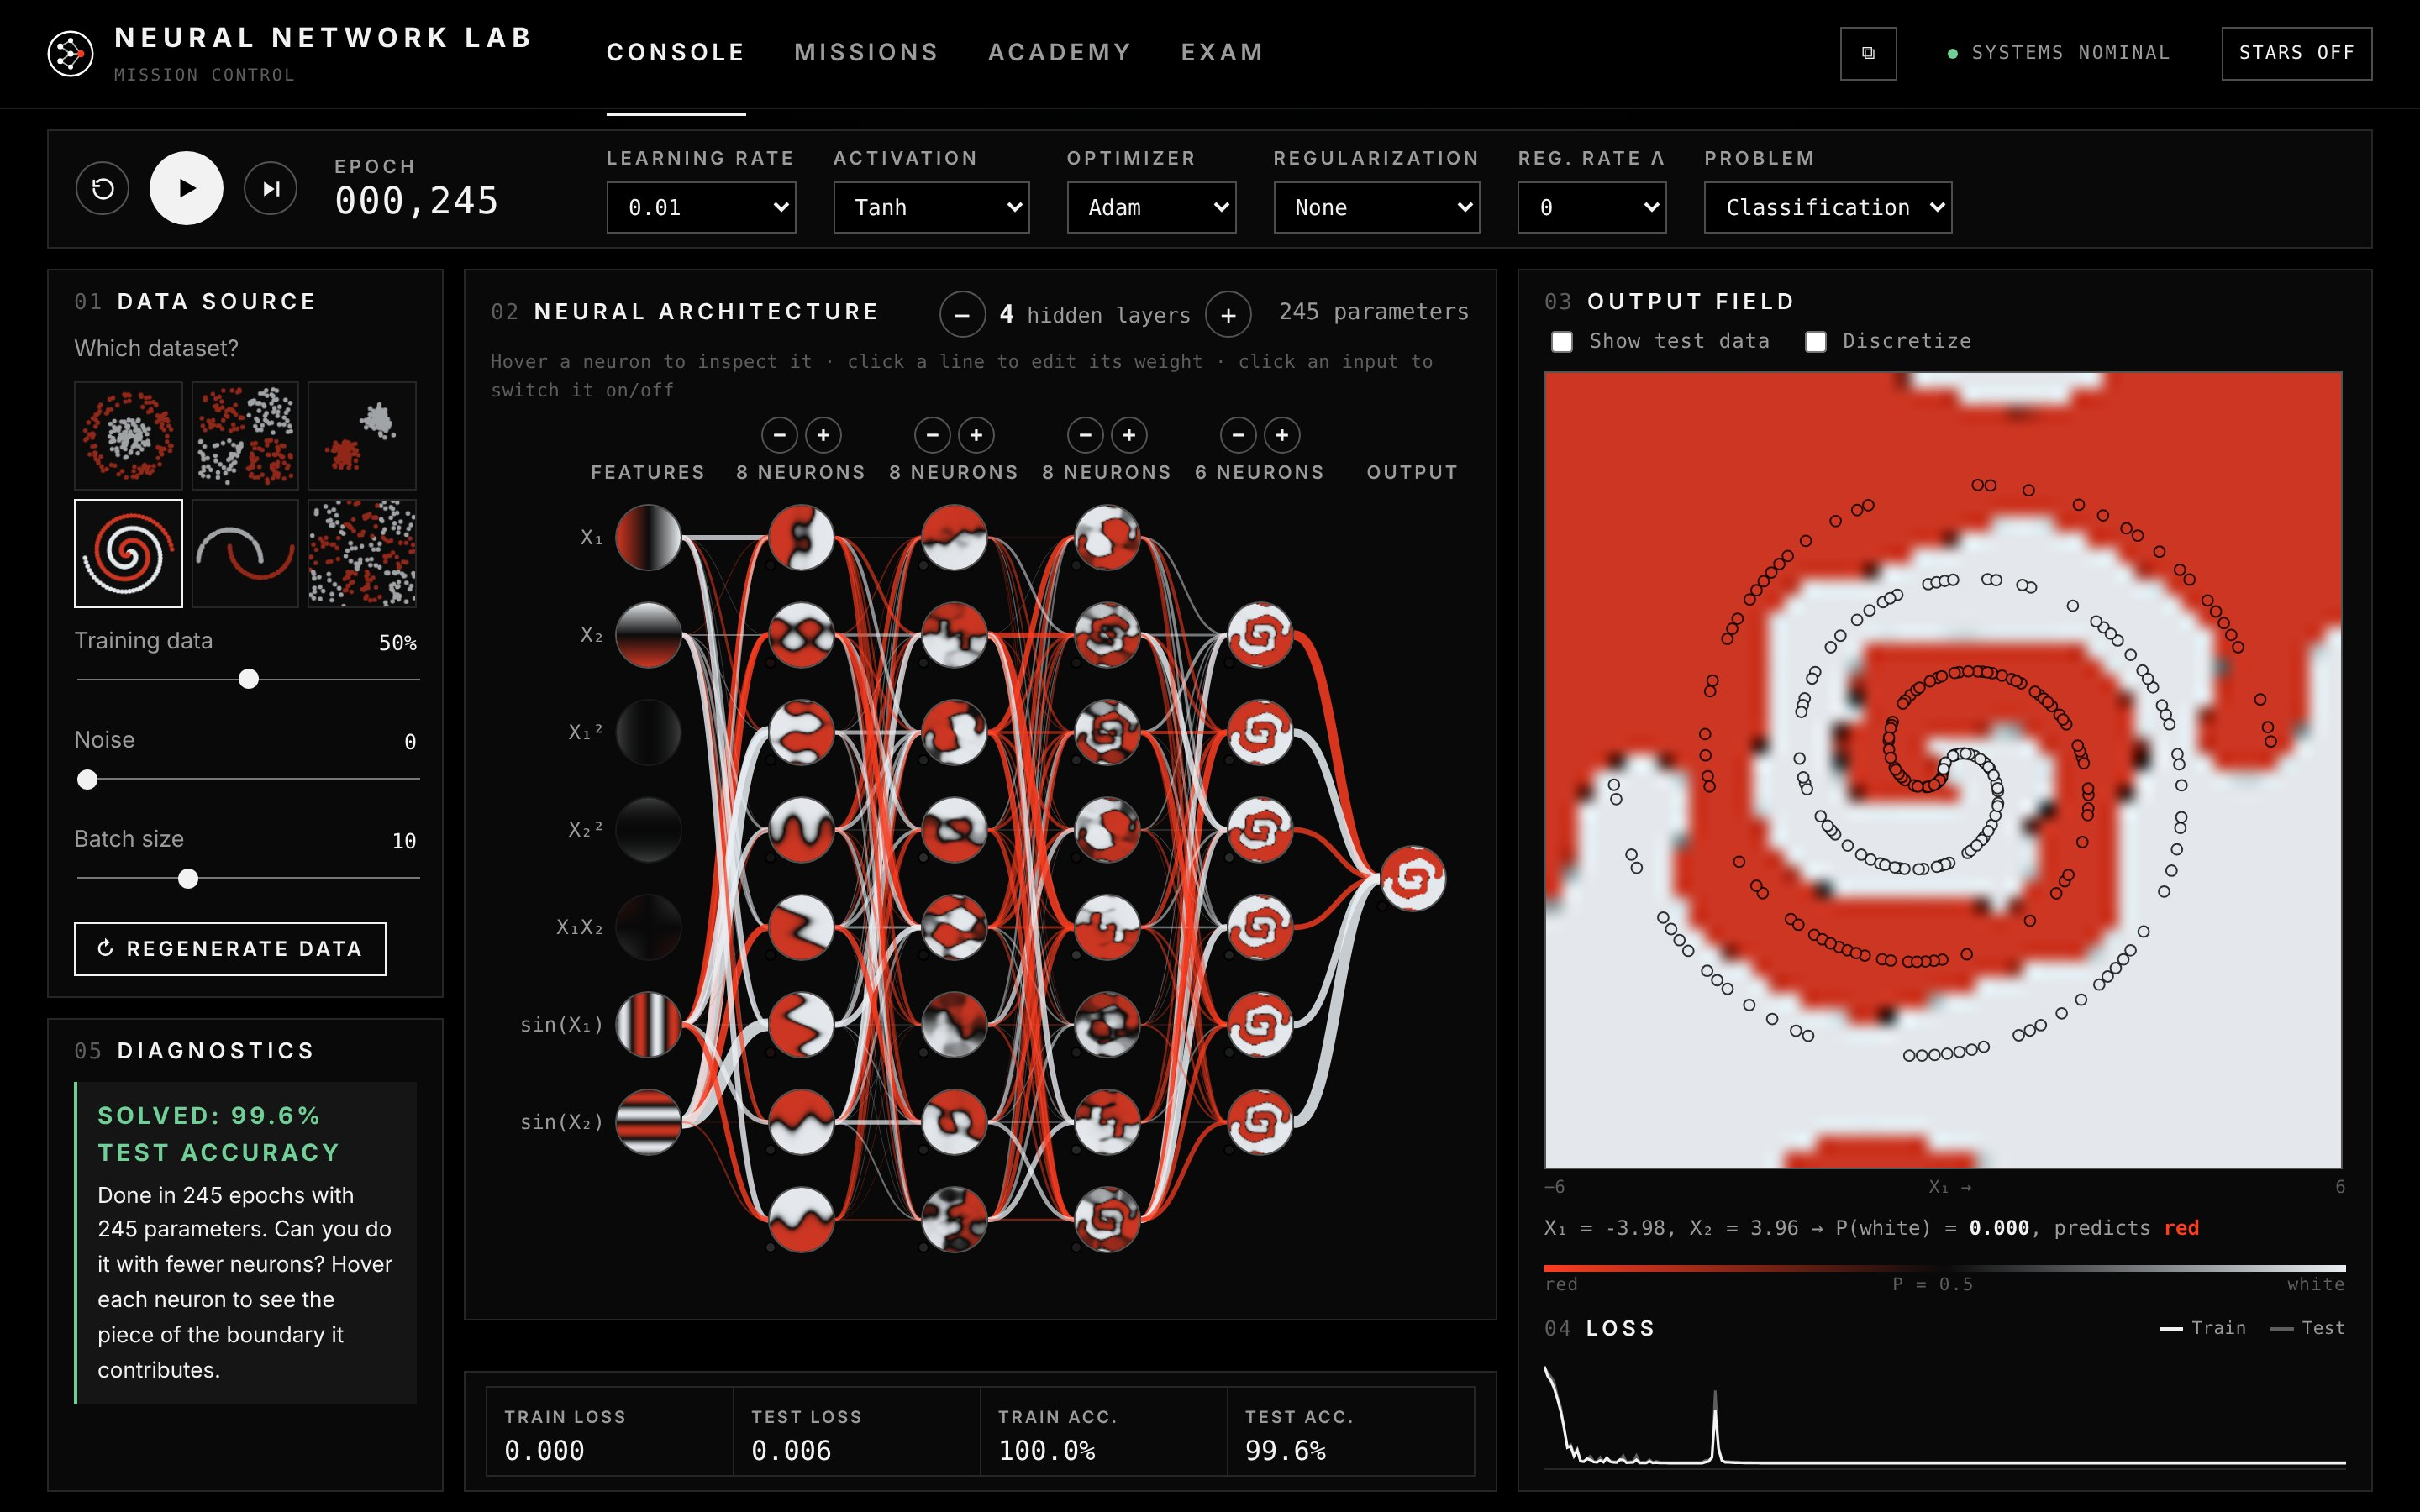
\includegraphics[width=\textwidth]{fig_ui.jpg}
\caption{The Console after training on the spiral data set (mission~10) with $\sin x_1$ and $\sin x_2$ added. Left: data set, sliders and diagnostics. Centre: the network, in which every circle is a neuron drawn as its own output over the input plane and every line is a weight (white positive, red negative; width proportional to $|w|$). Right: the network's output over the plane with the training points, and the loss curves.}\label{fig:ui}
\end{figure}

\paragraph{Visual encoding.} Every neuron is drawn as a small map of its activation over the $50 \times 50$ grid of input points, so the learner can see that first-layer neurons draw straight lines and later neurons combine them. Hovering a neuron enlarges its map on the output panel; hovering a weight shows its value, and clicking it opens an editor, so the learner can set a weight by hand and see the effect. Hovering the output map reports the predicted probability at that point.

\paragraph{Diagnostics.} After each epoch a small rule engine chooses one message (\cref{tab:rules}). The rules are deliberately simple and are checked in order; each names the cause and the remedy in plain language.

\begin{table}[!htbp]
\centering\small
\caption{Diagnostic rules, in the order they are checked.}\label{tab:rules}
\begin{tabularx}{\textwidth}{l >{\raggedright\arraybackslash}X}
\toprule
Message & Condition and explanation given \\
\midrule
Training blew up & Training loss is not finite or exceeds 50: the learning rate overshoots the minimum. \\
All-linear collapse & Linear activation with hidden layers on a non-linear data set with raw inputs: $W_2(W_1\mathbf{x} + \mathbf{b}_1) + \mathbf{b}_2$ is still linear. \\
One straight line is not enough & No hidden layer, raw inputs, non-linear data set, after 30 epochs: logistic regression draws one line; suggests a hidden layer or features. \\
Dead neurons & ReLU network in which at least 30\% of hidden neurons output 0 everywhere on the grid. \\
Overfitting & After 120 epochs, test loss is more than 15\% above its best while training loss is still falling. \\
Solved & Test accuracy at least 97\% (with a note if test loss is rising). \\
Barely learning & After 200 epochs the loss is above 85\% of its starting value. \\
\bottomrule
\end{tabularx}
\end{table}

\paragraph{Missions.} \Cref{tab:missions} lists the \nMissions{} missions. Each one loads a configuration and a short brief that poses a question; they move from a single neuron, through two ways to fix a failing linear model (features or a hidden layer), to common pitfalls and a final ``spiral'' challenge.

% =====================================================================
\section{The Academy}\label{sec:academy}

The Academy is a single page of seven lessons, each built around a widget the learner operates (\cref{tab:academy}). The backpropagation lesson (\cref{fig:bp}) runs one complete training step on a 2--2--1 network: the learner moves through nine stages, from the weighted sums to the parameter update, and every intermediate number is computed live from inputs and a target the learner can change, ending with a forward pass under the new weights that confirms the loss went down. The page closes with a searchable glossary of 30 terms and a 16-statement true/false quiz in which each answer is followed by its justification.

\begin{table}[!htbp]
\centering\small
\caption{Academy lessons and the statistical idea each one connects to.}\label{tab:academy}
\begin{tabularx}{\textwidth}{l >{\raggedright\arraybackslash}X >{\raggedright\arraybackslash}X}
\toprule
Lesson & Interactive widget & Connection to the course \\
\midrule
1. The neuron & Sliders for $w_1$, $w_2$, $b$ and the activation; live decision boundary and weight vector & A sigmoid neuron is logistic regression; log-odds are linear \\
2. Activation functions & Each function with its derivative; facts and trade-offs & Why linear layers collapse; vanishing gradients \\
3. Hidden layers & Three networks train side by side on the same data & Basis expansion versus learned features \\
4. Loss & Log loss and squared error with a draggable prediction & Negative log-likelihood; least squares as Gaussian likelihood \\
5. Gradient descent & Four loss surfaces, three optimisers, learning rate and noise; click to start & Conditioning and standardisation; local minima \\
6. Backpropagation & Nine-step, number-by-number training update & The chain rule \\
7. Overfitting & Two networks on 50 noisy points, with and without L2 & Bias--variance; ridge and lasso; validation \\
\bottomrule
\end{tabularx}
\end{table}

\begin{figure}[!htbp]
\centering
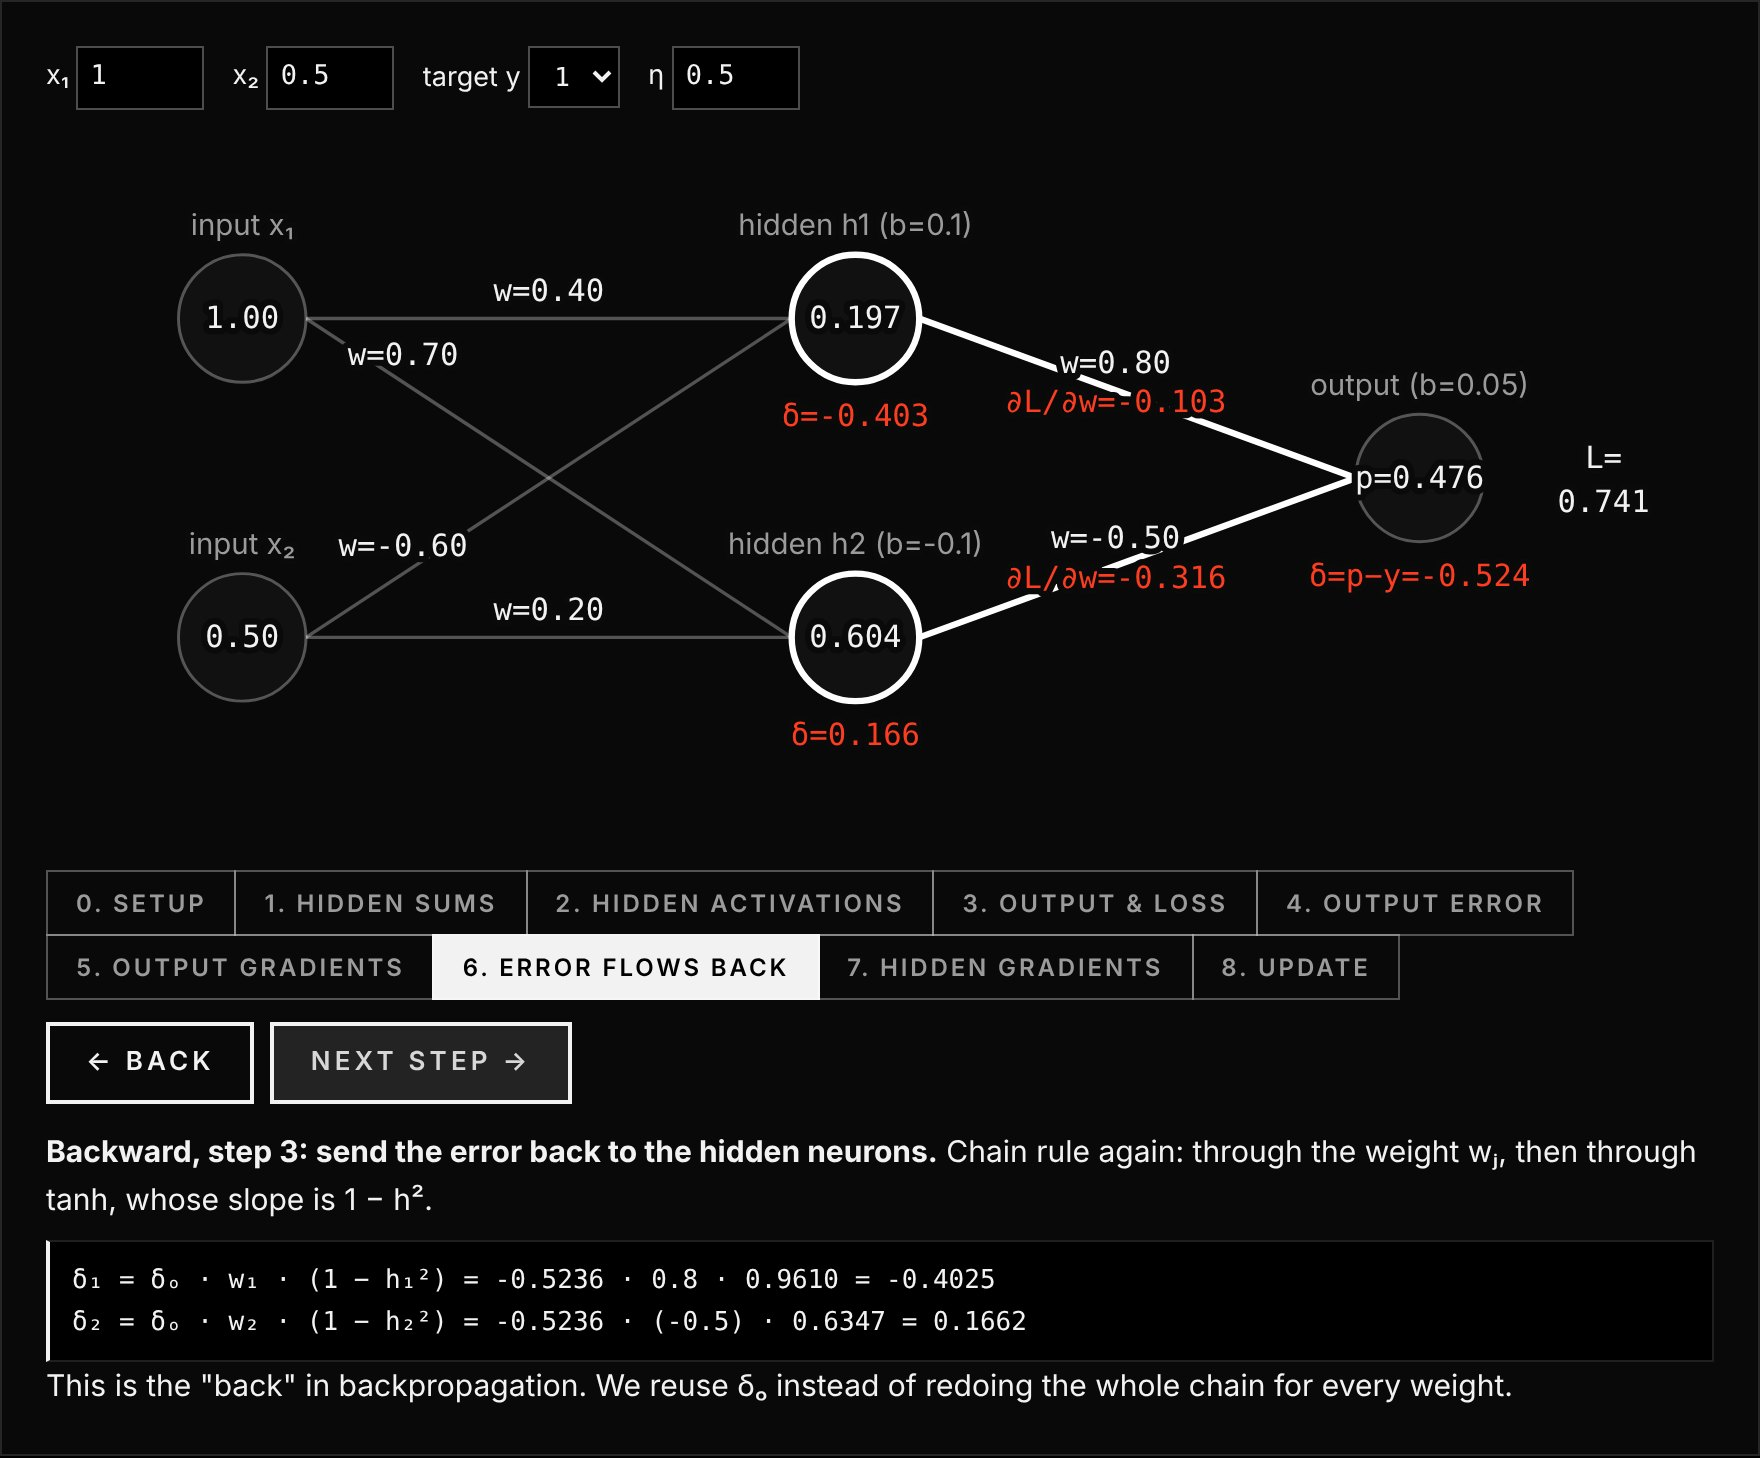
\includegraphics[width=0.82\textwidth]{fig_backprop.jpg}
\caption{The backpropagation lesson at step~6, ``Error flows back'': the output error $\delta_o = p - y$ has produced the gradients of the output weights (red) and is being sent back through each connection and the slope of tanh to give the hidden errors $\delta_1, \delta_2$.}\label{fig:bp}
\end{figure}

% =====================================================================
\section{Technical validation}\label{sec:validation}

All experiments below run the website's own modules (\code{js/nn.js}, \code{js/data.js}, \code{js/missions.js}) under Node.js with the same training procedure as the Console and seeded random numbers. Each experiment is repeated with \nSeeds{} seeds for the network's initial weights and the shuffling order; results are reported as mean $\pm$ standard deviation. The complete benchmark took \runtime{} seconds.

\subsection{Gradient check}\label{sec:gradcheck}
For every activation and both tasks, a 3--5--4--1 network with random weights was given one random example, and each analytic gradient was compared with a central finite difference ($h = 10^{-6}$) of the loss. \Cref{tab:grad} reports the largest relative error $|g_a - g_n| / (|g_a| + |g_n|)$. Across \gcParams{} parameters the maximum was $\gcMax$, consistent with finite-difference rounding error and confirming that the backpropagation equations are implemented correctly.

\begin{table}[!htbp]
\centering\small
\caption{Gradient check: largest relative error between analytic and numerical gradients.}\label{tab:grad}
\begin{tabular}{l l r r}
\toprule
Activation & Task & Parameters & Max.\ relative error \\
\midrule
\inputtab{tab_gradcheck.tex}
\bottomrule
\end{tabular}
\end{table}

\subsection{Missions}
\Cref{tab:missions} reports each mission's outcome with its default settings after 400 epochs (1{,}000 for the spiral). The missions behave as their briefs say. The linear model on the circle stays near chance, and it is fixed equally well by engineered features or by four tanh neurons. Three linear hidden layers do no better than no hidden layer. A learning rate of~3 gives unstable, seed-dependent results. The overfitting mission gives a large gap between training and test performance, and the spiral is solved by a four-layer network with Adam ($\spiralAcc \pm \spiralSd$\% test accuracy, \spiralParams{} parameters).

\begin{table}[!htbp]
\centering\footnotesize
\setlength{\tabcolsep}{4pt}
\caption{Missions with their default settings. Test accuracy is the mean $\pm$ standard deviation over \nSeeds{} seeds after the stated number of epochs; ``$\geq$95\%'' counts seeds that reached 95\% test accuracy at some epoch. Mission~11 is regression and reports test mean squared error.}\label{tab:missions}
\begin{tabularx}{\textwidth}{r >{\raggedright\arraybackslash}X l l l l r l c}
\toprule
\# & Mission & Data & Hidden & Act. & Optimiser & Par. & Test acc.\ (\%) & $\geq$95\% \\
\midrule
\inputtab{tab_missions.tex}
\bottomrule
\end{tabularx}
\end{table}

\subsection{Model capacity: features versus hidden layers}
\Cref{tab:capacity} and \cref{fig:capacity} compare four models on four data sets, each trained for 400 epochs with SGD ($\eta = 0.03$). Logistic regression on $(x_1, x_2)$ reaches \capCircleLin\% on the circle and \capXorLin\% on XOR, close to chance, because its boundary is a single line. Adding the engineered features $x_1^2$, $x_2^2$ and $x_1x_2$ raises both to \capCircleFeat\%, while a hidden layer of four tanh neurons, which learns its own features, reaches \capCircleTanh\% and \capXorTanh\%. Four \emph{linear} hidden neurons give \capCircleLinHid\% and \capXorLinHid\%: as the algebra predicts, they are no better than logistic regression.

\begin{table}[!htbp]
\centering\small
\caption{Test accuracy (\%, mean $\pm$ sd over \nSeeds{} seeds) of four models on four data sets.}\label{tab:capacity}
\begin{tabular}{l c c c c}
\toprule
Model & Gaussian & Circle & XOR & Two moons \\
\midrule
\inputtab{tab_capacity.tex}
\bottomrule
\end{tabular}
\end{table}

\begin{figure}[!htbp]
\centering
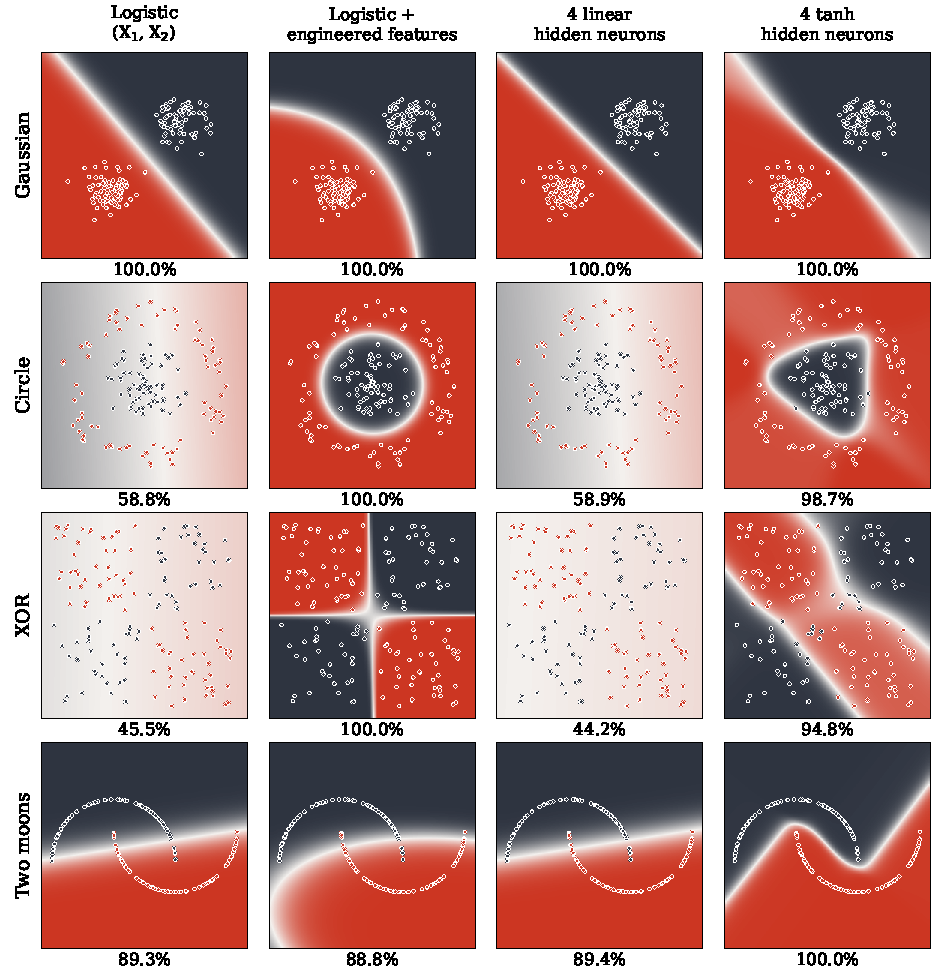
\includegraphics[width=0.9\textwidth]{fig_capacity.pdf}
\caption{Output of each model over the input plane after training (first seed), with training points; red is class $-1$, dark is class $+1$. The number under each panel is the mean test accuracy over \nSeeds{} seeds.}\label{fig:capacity}
\end{figure}

\subsection{Overfitting and L2 regularisation}
To reproduce the Academy's overfitting lesson, a 2--8--8--1 tanh network was trained with Adam ($\eta = 0.02$) for 1{,}600 epochs on 50 points from the two-moons data with noise $\nu = 0.32$, and tested on 400 further points, for six values of the L2 strength $\lambda$ (\cref{fig:overfit}). Without a penalty the training loss falls to \ofTrainNoReg{} while the test loss, which was lowest (\ofBestNoReg{} on average) early in training, rises to \ofTestNoReg{}; the sum of squared weights grows to \ofWsqNoReg{}. With $\lambda = 0.01$ the training loss stays at \ofTrainLtwo{}, the test loss ends at \ofTestLtwo{} and the squared weights stay at \ofWsqLtwo{}. Test loss is U-shaped in $\lambda$, lowest at $\lambda = \ofBestLam$ (\ofBestLamLoss{}): too little penalty leaves high variance and too much adds bias, the trade-off covered for ridge regression in the course.

\begin{figure}[!htbp]
\centering
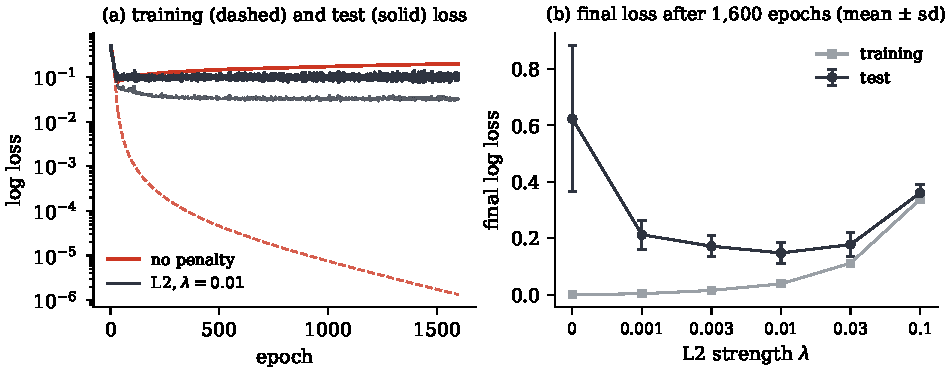
\includegraphics[width=\textwidth]{fig_overfit.pdf}
\caption{Overfitting on 50 noisy points. (a) Training and test loss over epochs for one seed, without a penalty and with L2 ($\lambda = 0.01$). (b) Final training and test loss against $\lambda$, mean $\pm$ sd over \nSeeds{} seeds.}\label{fig:overfit}
\end{figure}

\subsection{Learning rate}
\Cref{tab:lr} and \cref{fig:lr} show plain SGD on the circle with the default 2--4--2--1 tanh network for 300 epochs at eight learning rates. A rate of 0.001 barely moves the loss (\lrSlow{}); the lowest final loss is at $\eta = \lrBest$ (\lrBestLoss{}); at $\eta = 3$ the loss is erratic and at $\eta = \lrDivFirst$ some runs diverge.

\begin{table}[!htbp]
\centering\small
\caption{Final training log loss after 300 epochs (mean over non-diverged seeds) and the number of seeds whose loss was not finite or exceeded 5.}\label{tab:lr}
\begin{tabular}{r r r}
\toprule
Learning rate $\eta$ & Final loss & Diverged \\
\midrule
\inputtab{tab_lr.tex}
\bottomrule
\end{tabular}
\end{table}

\begin{figure}[!htbp]
\centering
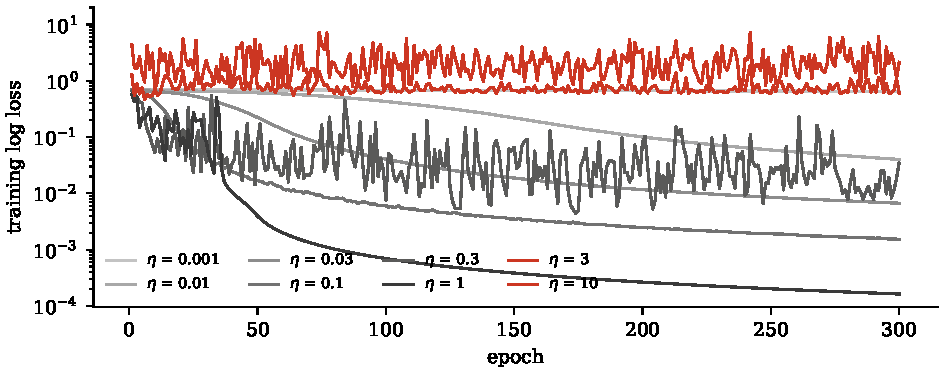
\includegraphics[width=\textwidth]{fig_lr.pdf}
\caption{Training loss over epochs for eight learning rates (first seed); red curves are the rates that are too large.}\label{fig:lr}
\end{figure}

\subsection{Speed and browser testing}
In Node.js one epoch on 250 training points took \msSmall{}~ms for the default \pSmall-parameter network and \msLarge{}~ms for a \pLarge-parameter spiral network; recomputing all neuron maps (2{,}500 forward passes) took \gridMs{}~ms. Training one epoch per animation frame therefore leaves most of each frame for drawing. Both pages were loaded in headless Chrome at $1280\times720$, $1366\times768$, $1440\times900$ and $1920\times1080$ pixels and on a $390\times844$ phone viewport. In every case there were no script errors, and on the desktop sizes the Console's content fitted the window without scrolling.

% =====================================================================
\section{Limitations}\label{sec:limits}

The networks are small and the data are two-dimensional, which is what makes every neuron drawable; the site does not show convolutional, recurrent or attention-based networks, and lessons learned on toy data do not all carry over to high-dimensional problems. The engine uses double-precision JavaScript arithmetic on the main thread, so very large networks would slow the animation. The diagnostic rules are heuristics with fixed thresholds: they can miss a problem, or describe a correct run too cautiously. Accuracy in the Console is measured on a single random split, not by cross-validation. Finally, the site has not yet been evaluated with learners, so its educational benefit is a design goal rather than a measured result.

% =====================================================================
\section{Conclusion}

Neural Network Lab lets a learner train a neural network in the browser, see what every neuron computes at every step, and read why the network succeeds or fails. By tying each behaviour to a statistical idea---logistic regression, likelihood, basis expansion, the bias--variance trade-off and ridge and lasso penalties---it is meant to help students who learn neural networks after a statistics course see the neural network as an extension of models they already understand. The engine's gradients are verified numerically, and every result in this report is regenerated from the site's own code.

\paragraph{Availability.} The website is at \siteurl{} and the source code, benchmark scripts and this report's \LaTeX{} source are at \url{https://github.com/sahiljangra12/neural-network-lab}. To reproduce the results: \code{node tools/benchmark.mjs}, then \code{python3 tools/figures.py}, then compile \code{paper/neural\_network\_lab.tex}.

\paragraph{Acknowledgements.} This project was inspired by \courseName{} at Johns Hopkins University, taught by \profName{} \citep{asda2026}. Its treatment of likelihood, logistic regression, regularisation and model selection shaped the Academy's lessons and missions. The interface was also inspired by TensorFlow Playground \citep{smilkov2017playground}. Any errors are the author's own.

\bibliographystyle{plainnat}
\bibliography{references}

\end{document}
